% Construction (perspective cavalière) : le plan (ABC) est le parallélogramme
% (0 ; 0), (6 ; 0), (7,6 ; 2), (1,6 ; 2). H = (3,2 ; 0,9), M = (5,4 ; 1,5),
% et S = (3,2 ; 3,7), à la verticale de H sur le dessin.
% [SH] est perpendiculaire au plan : c'est la plus courte distance de S au plan.
\begin{tikzpicture}[scale=0.78]
  \draw (0, 0) -- (6, 0) -- (7.6, 2) -- (1.6, 2) -- cycle;
  \coordinate (H) at (3.2, 0.9);
  \coordinate (M) at (5.4, 1.5);
  \coordinate (S) at (3.2, 3.7);
  \draw[dashed] (S) -- (H);
  \draw (S) -- (M);
  \draw[dashed] (H) -- (M);
  \draw (3.2, 1.18) -- (3.48, 1.18) -- (3.48, 0.9);
  \foreach \p in {H, M, S} \fill (\p) circle (1.6pt);
  \node[above] at (S) {$S$};
  \node[below right] at (H) {$H$};
  \node[below right] at (M) {$M$};
  \node[left] at (3.2, 2.4) {$\dfrac{\sqrt{21}}{2}$};
  \node[right] at (7, 0.4) {$(ABC)$};
\end{tikzpicture}
